\documentclass[12pt]{article}


%%%%%%%%%%%%%%%%%%%%%%%%%%%%%baliky%%%%%%%%%%%%%%%%%%%%%%%%%%%%%%%%%%%%%%%%%%

\usepackage{graphicx} %vkladanie grafiky
\usepackage{caption}  %vkladanie a nastavenie popiskov obrázkov
\usepackage{calc}     %možnos vkladania parametrov vo forme výrazov
\usepackage{amsmath}  %AMS-TeXovský balík pre sádzanie vzorcov
\usepackage{amssymb}  %AMS-TeXovské matematické symboly
\usepackage{amsfonts} %AMS fonty
\usepackage{bm}       %tuèné matematické symboly
\usepackage{url}      %tvorba internetových odkazov 
\usepackage{longtable}%tvorba tabu¾ky na viac ako jednu stranu
\usepackage{titlesec} %nastavenie nazvu kapitoly
\usepackage{multirow} %zlucovanie riadkov 
\usepackage{parcolumns} % balik na pisanie textu v stlpcoch
\usepackage{relsize}  %velkost matematickeho fontu
\usepackage{epsfig}   %vkladanie obrazkov do rovnic



% *************** Ve¾kos textovej plochy na stránke****************
\addtolength{\hoffset}{-1cm}     % vzdialenost textu od praveho okraja papiera
\addtolength{\voffset}{-2cm}     % vzdialenost textu od horneho okraja papiera
\addtolength{\textwidth}{2cm}    % velkost sirky textu (textwidth =12.65cm)
\addtolength{\textheight}{3.5cm}   % velkost vysky textu (textwidth =20.91cm)
\linespread{1.3}      %riadkovanie 1,5      
\frenchspacing        %štandardná medzera za každou bodkou v texte

%%%%%%%%%%%%%%%%%%%%%%%%%%% Vlastne prikazy %%%%%%%%%%%%%%%%%%%%%%%%%%%%%%%%%%%
\newcommand{\psid}{\psi^{\dagger}}

%prikaz na pociatocne udaje - prvy parameter: poradove cislo, druhy parameter: odpovedajuca casti ucinku, treti parameter: vertex factor a stvrty parmeter je symmetry coefficient.
\newcommand{\pociat}[4]{
\begin{table}[!ht]
\begin{tabular}{|c |c @{\hspace{2cm}} l}
\cline{1-1}
& \\ [-2ex]
\LARGE $#1 .$ & &{\large Vertex factor:}\qquad $#3$ \\ [0.5ex]
$#2$ & & {\large Symmetry coefficient:} \qquad $#4$ \\ \cline{1-1} 
\end{tabular}
\end{table}}

% nastavenie obrazka grafu - prvy parameter je nazov obrazku aj s priponou a druhy je vysledok integralu
\newcommand{\obr}[2]{\begin{minipage}{0.4\textwidth}
\includegraphics[width=\linewidth,keepaspectratio=true]{figure/#1}
\end{minipage}%%% to prevent a space
\begin{minipage}{0.6\textwidth}
\begin{displaymath} 
= #2 \nonumber
\end{displaymath}
\null
\par\xdef\tpd{\the\prevdepth}
\end{minipage}
}

% renormalizacne konstanty - parameter oznacuje cislo samotnej konstanty
\newcommand{\zcon}[1]{
Z_{#1} \hspace{0.5cm} \Rightarrow \hspace{0.5cm} Z_{#1} = Z_{#1} }

%%%%%%%%%%%%%%%%%%%%%%%%%%%%%%%%%%%%%%%%%%%%%%%%%%%%%%%%%%%%%%%%%%%%%%%%%%%%%%%

\begin{document}

\section*{DP 1 loop graphs}

Action Functional:
\begin{eqnarray}
S_R &=& \psid (-Z_1\partial_t - Z_4(\mathbf{v}\cdot\nabla) - a Z_5 (\nabla\cdot
{\mathbf v})+ Z_2 D \nabla^2 - Z_3 D \tau) \psi +  \nonumber \\
 &+& \frac{D \lambda}{2} \Big[ Z_6 (\psid)^2 \psi - Z_7 \psid \psi^2 \Big] 
 +Z_8 \frac{u_2}{2D} \psid \psi \mathbf{v}^2  - \frac{1}{2} \mathbf{ v} D^{-1}_v  \mathbf{v}. 
\end{eqnarray}


Green function in the model

\begin{eqnarray}
  \langle \psid \psi \rangle_{1-ir} &=& i\omega Z_1 - D p^2 Z_2 -
   D \tau Z_3 + \raisebox{-0.7ex}{\epsfysize=0.9truecm \epsffile  {figure/obr1.eps}} 
  + \nonumber \\ 
  & + & \frac{1}{2}  \raisebox{-0.7ex}{\epsfysize=0.9truecm \epsffile{figure/obr2.eps}} + 
  \frac{1}{2}  \raisebox{-1.5ex}   {\epsfysize=1.5truecm \epsffile{figure/obr3.eps}}
\end{eqnarray}

\begin{eqnarray}
  \langle \psid \psi {\mathbf v} \rangle_{1-ir} &=&  -i p_j Z_4 -i a q_j Z_5 + 
  \raisebox{-2.5ex}{\epsfysize=1.2truecm \epsffile{figure/obr4.eps}}+
  \raisebox{-2.5ex}{\epsfysize=1.2truecm \epsffile{figure/obr5.eps}}+ \nonumber \\
  & + & \raisebox{-0.7ex}{\epsfysize=0.9truecm \epsffile{figure/obr6.eps}} +
  \raisebox{-0.7ex}{\epsfysize=0.9truecm \epsffile{figure/obr7.eps}}
\end{eqnarray}

\begin{eqnarray}  
  \langle \psid \psid \psi \rangle_{1-ir} &=& D \lambda Z_6 +
   2 \raisebox{-2.5ex}{\epsfysize=1.2truecm \epsffile{figure/obr8.eps}}+ 
  \raisebox{-2.5ex}{\epsfysize=1.2truecm \epsffile{figure/obr9.eps}}+ \nonumber \\
  & + & 2 \raisebox{-3ex}{\epsfysize=1.2truecm \epsffile{figure/obr10.eps}}
\end{eqnarray}

\begin{eqnarray}  
  \langle \psid \psi \psi \rangle_{1-ir}  & = &
  -D \lambda Z_7 +  2 \raisebox{-2.5ex}{\epsfysize=1.2truecm \epsffile{figure/obr11.eps}}+ 
  \raisebox{-2.5ex}{\epsfysize=1.2truecm \epsffile{figure/obr12.eps}}+ \nonumber\\
  & + & 2 \raisebox{-3ex}{\epsfysize=1.2truecm \epsffile{figure/obr13.eps}}
\end{eqnarray}  
  
\begin{eqnarray}  
  \langle \psid \psi {\mathbf v}^2 \rangle_{1-ir} &=& \frac{u_2}{D} \delta_{ij} Z_8 + 
  \raisebox{-2.5ex}{\epsfysize=1.2truecm \epsffile{figure/obr14.eps}} + 
  \raisebox{-2.5ex}{\epsfysize=1.2truecm \epsffile{figure/obr15.eps}} + \nonumber \\
  &+& \raisebox{-2.5ex}{\epsfysize=1.2truecm \epsffile{figure/obr16.eps}} +
  \raisebox{-2.5ex}{\epsfysize=1.2truecm \epsffile{figure/obr17.eps}} +
  \raisebox{-2.5ex}{\epsfysize=1.2truecm \epsffile{figure/obr18.eps}} + \nonumber \\
  &+& \raisebox{-2.5ex}{\epsfysize=1.2truecm \epsffile{figure/obr19.eps}} +
  \raisebox{-2.5ex}{\epsfysize=1.2truecm \epsffile{figure/obr20.eps}} + 
  \raisebox{-0.7ex}{\epsfysize=0.8truecm \epsffile{figure/obr21.eps}} \nonumber 
\end{eqnarray}


\newpage

\begin{table}[!ht]
\centering
\begin{tabular}{c c}
\multicolumn{2}{c}{ Propagators }\\
\hline
\multirow{2}{*}{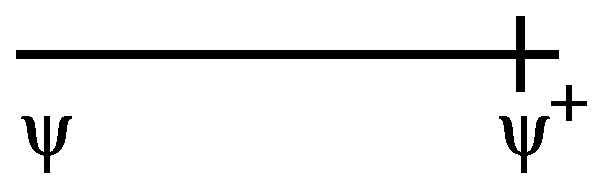
\includegraphics[width=3.5cm]{figure/prop1.eps}} &  $=\frac{1}{-i\omega + D(k^2+\tau)}$   \\
& \\
\multirow{2}{*}{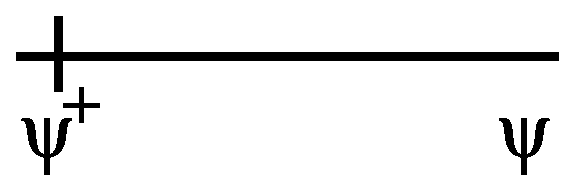
\includegraphics[width=3.5cm]{figure/prop2.eps}} &  $=\frac{1}{i\omega + D(k^2+\tau)} $  \\
& \\
\multirow{2}{*}{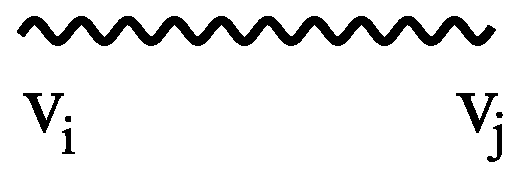
\includegraphics[width=3.5cm]{figure/prop3.eps}} & $=\frac{g_1 u_1 D^3 k^{4-d-y-\eta}}{\omega^2+u_1^2D^2 (k^{2-\eta})^2}(P_{ij}^k +\alpha Q_{ij}^k)$ \\
& \\
\hline
\multicolumn{2}{c}{ Vertices }\\
\hline
\multirow{4}{*}{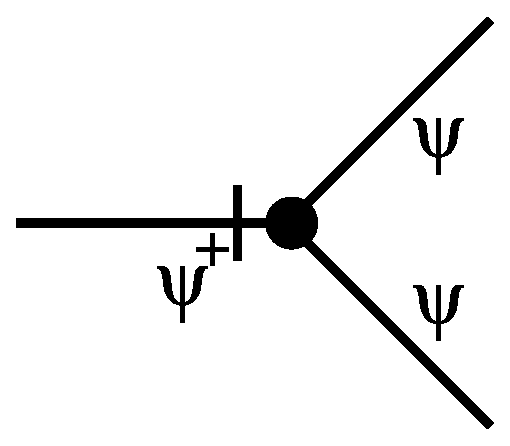
\includegraphics[width=2.5cm]{figure/vert1.eps}} & \\
& \multirow{2}{*}{$= - D \lambda$}\\
& \\
& \\[1ex]
\multirow{4}{*}{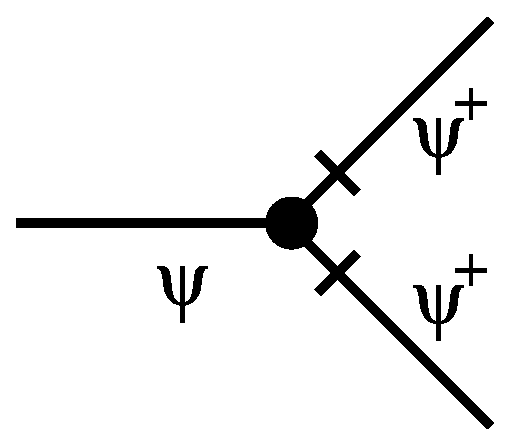
\includegraphics[width=2.5cm]{figure/vert2.eps}} & \\
& \multirow{2}{*}{$=D \lambda$}\\
& \\
& \\[1ex]
\multirow{4}{*}{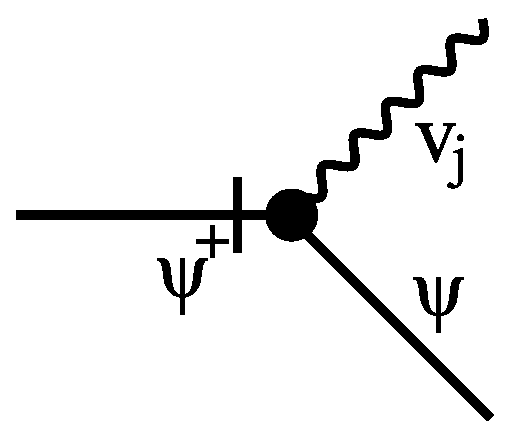
\includegraphics[width=2.5cm]{figure/vert3.eps}} & \\
& \multirow{2}{*}{$=-i p_j -iaq_j$}\\
& \\
& \\[1ex]
\multirow{4}{*}{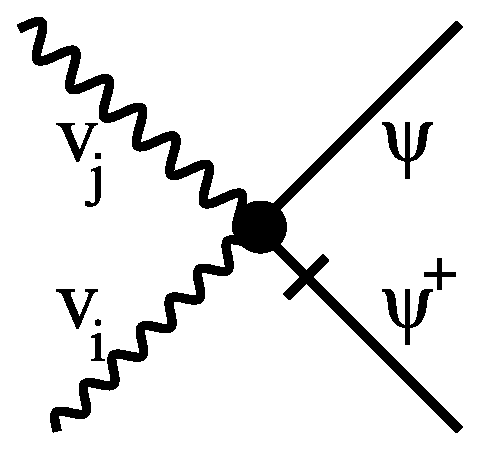
\includegraphics[width=2.5cm]{figure/vert4.eps}} &  \\
& \multirow{2}{*}{$= \frac{u_2}{D} \delta_{ij} $}\\
& \\
& \\[1ex]
\end{tabular}
\end{table} 

$p$ - momentum of the $\psi$ and $q$ - momentum of the ${\bf v}$ in vertex $\psid \psi {\bf v}$

\begin{itemize}
\item effective charge $g_2$
  \begin{equation}
    g_2 \equiv \lambda^2
  \end{equation}
\item Redefinition of charges $g_1$ and $g_2$
  \begin{equation}
    \frac{g_1}{16 \pi^2} \rightarrow  g_1 \hspace{2cm} \frac{g_2}{16 \pi^2} \rightarrow g_2 \nonumber
  \end{equation}
\item
   \begin{equation}
      d = 4 - \epsilon \nonumber
  \end{equation}
\item 
  \begin{equation}
     I_\epsilon = \frac{S_d}{(2\pi)^d} m^{ \epsilon} \quad I_y = \frac{S_d}{(2\pi)^d} m^{-y}
  \end{equation}
\end{itemize}

\newpage 

%%%%%%%%%%%%%%%%%%%%%%%%%%%%%%%%%%%%%%%%%%
\pociat{1}{\psid  \psi}{1}{1}

\begin{minipage}{0.4\textwidth}
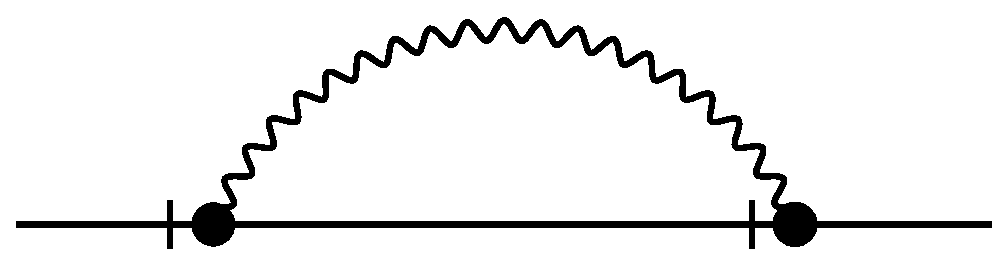
\includegraphics[width=\linewidth,keepaspectratio=true]{figure/obr1.eps}
\end{minipage}%%% to prevent a space
\begin{minipage}{0.6\textwidth}
\begin{eqnarray*}
    &-& \textstyle \frac{g_1 D p^2 I_y}{2d(1+u_1)} \frac{1}{y}\left[ d-1 + 
    \alpha - \frac{2\alpha}{1+u_1}+ \frac{\alpha a(1-a)}{1+u_1}\left(\frac{4}{1+u_1}-d \right)\right] \\ 
    &-& i \omega \frac{g_1 \alpha a (1-a) I_y}{2(1+u_1)^2} \frac{1}{y} +
     \tau D \frac{g_1 \alpha a (1-a) I_y}{2(1+u_1)^2} \frac{1}{y}
\end{eqnarray*}
\null
\par\xdef\tpd{\the\prevdepth}
\end{minipage}

%\begin{eqnarray*}
%\zcon{1} &+& \frac{g_1 \alpha a (1-a)}{(1+u_1)^2}\frac{1}{y} \\
%\zcon{2} &-& \frac{g_1}{4(1+u_1)}\frac{1}{y}\left[ 3 +
% \alpha\left(1 - \frac{2}{1+u_1}- \frac{4a(1-a)u_1}{(1+u_1)^2}\right)%\right] \\
%\zcon{3} &+& \frac{g_1 \alpha a (1-a)}{(1+u_1)^2}\frac{1}{y}
%\end{eqnarray*}

%%%%%%%%%%%%%%%%%%%%%%%%%%%%%%%%%%%%%%%%%%
\pociat{2}{\psid  \psi}{-D^2 \lambda^2}{\frac{1}{2}}

\obr{obr2.eps}{\frac{I_\epsilon}{2D} \left[ \frac{i \omega}{2 D} -\tau -p^2 \frac{d-2}{2d} \right ] \frac{1}{\epsilon}}

%\begin{eqnarray*}
%\zcon{1} &+& \frac{g_2}{4\epsilon}  \\
%\zcon{2} &+& \frac{g_2}{8\epsilon} \\
%\zcon{3} &+& \frac{g_2}{2\epsilon} \\
%\end{eqnarray*}

%%%%%%%%%%%%%%%%%%%%%%%%%%%%%%%%%%%%%%%%%%
\pociat{3}{\psid \psi}{\frac{u_2}{D} \delta_{ij}}{\frac{1}{2}}

\obr{obr3.eps}{\frac{g_1 D^2 (d-1 + \alpha)}{2 }\frac{S_d}{(2\pi)^d}\int\limits_{0}^{\sqrt{\tau}\Lambda} dk \quad  k^{2-y -1}}

\newpage
%%%%%%%%%%%%%%%%%%%%%%%%%%%%%%%%%%%%%%%%%%
\pociat{4}{\psid \psi {\mathbf v}}{-D^2 \lambda^2}{1}

\obr{obr4.eps}{\frac{- i I_\epsilon}{4 d D^2} \frac{1}{\epsilon} [2 p_j+q_j(ad+3-d)]}

%\begin{eqnarray*}
%\zcon{4} &+& \frac{g_2}{4 \epsilon} \\
%\zcon{5} &+& \frac{g_2}{\epsilon} \frac{4a-1}{8a}
%\end{eqnarray*}

%%%%%%%%%%%%%%%%%%%%%%%%%%%%%%%%%%%%%%%%%%
\pociat{5}{\psid \psi {\mathbf v}}{1}{1}

\obr{obr5.eps}{\textstyle \frac{ i g_1 \alpha I_y}{2 (1+u_1)^2}\frac{1}{y} \left[(p_j+ a q_j)\left(\frac{1}{d}+a-a^2\right) - \frac{2a(1-a)}{(1+u_1)d} (2 p_j +q_j) \right] }

%\begin{eqnarray*}
%\zcon{4} &+&  \frac{g_1 \alpha }{4 (1+u_1)^2}\frac{1}{y} \left[ 1 + 4a(1 -a) \left(1 -\frac{1}{1+u_1} \right) \right] \\
%\zcon{5} &+&  \frac{g_1 \alpha }{4 (1+u_1)^2}\frac{1}{y} \left[ 1 + 2 (1 -a) \left(2a -\frac{1}{1+u_1} \right)\right]
%\end{eqnarray*}

%%%%%%%%%%%%%%%%%%%%%%%%%%%%%%%%%%%%%%%%%%
\pociat{6}{\psid \psi {\mathbf v}}{\frac{u_2}{D} \delta_{ij}}{1}

\obr{obr6.eps}{-\frac{i p_j g_1 D I_y}{2 d (1+u_1)}\frac{1}{y}\left[d -1 + \alpha \left(1 - \frac{2 a}{1+u_1}\right) \right]}

%\begin{eqnarray*}
%\zcon{4} - \frac{ g_1 u_2}{4 (1+u_1)}\frac{1}{y}\left[3 + \alpha \left(1 - \frac{2 a}{1+u_1}\right) \right]
%\end{eqnarray*}

\newpage
%%%%%%%%%%%%%%%%%%%%%%%%%%%%%%%%%%%%%%%%%%
\pociat{7}{\psid \psi {\mathbf v}}{\frac{u_2}{D}\delta_{ij}}{1}

\obr{obr7.eps}{-\frac{i (p_j+q_j) g_1 D I_y}{2d(1+u_1)}\frac{1}{y}\left[d - 1 + \alpha - \frac{2\alpha (1-a)}{1+u_1}\right]}

%\begin{eqnarray*}
%\zcon{4} &-& \frac{ g_1 u_2}{4(1+u_1)}\frac{1}{y}\left[3 + \alpha - \frac{2\alpha (1-a)}{1+u_1}\right] \\
%\zcon{5} &-& \frac{ g_1 u_2}{4a(1+u_1)}\frac{1}{y}\left[3 + \alpha - \frac{2\alpha (1-a)}{1+u_1}\right]
%\end{eqnarray*}

%%%%%%%%%%%%%%%%%%%%%%%%%%%%%%%%%%%%%%%%%%
\pociat{8}{(\psid)^2 \psi}{-D^3 \lambda^3}{1}

\obr{obr8.eps}{\frac{I_\epsilon}{4D^2} \frac{1}{\epsilon}}

%\begin{eqnarray*}
%\zcon{6} + \frac{g_2}{\epsilon}
%\end{eqnarray*}

%%%%%%%%%%%%%%%%%%%%%%%%%%%%%%%%%%%%%%%%%%
\pociat{9}{(\psid)^2 \psi}{D\lambda}{1}

\obr{obr9.eps}{\frac{\alpha g_1 I_y (1-a)^2}{2(1+u_1)}\frac{1}{y}}

%\begin{eqnarray*}
%\zcon{6} - \frac{g_1 \alpha (1-a)^2}{(1+u_1)}\frac{1}{y}
%\end{eqnarray*}

\newpage
%%%%%%%%%%%%%%%%%%%%%%%%%%%%%%%%%%%%%%%%%%
\pociat{10}{(\psid)^2 \psi}{D\lambda}{1}

\obr{obr10.eps}{-\frac{\alpha g_1 a (1-a) I_y}{2(1+u_1)^2}\frac{1}{y}}

%\begin{eqnarray*}
%\zcon{6} + \frac{2 \alpha a (1-a) g_1}{(1+u_1)^2}\frac{1}{y}
%\end{eqnarray*}

%%%%%%%%%%%%%%%%%%%%%%%%%%%%%%%%%%%%%%%%%%
\pociat{11}{\psid \psi^2}{(D\lambda)^3}{1}

\obr{obr11.eps}{\frac{I_\epsilon}{4D^2} \frac{1}{\epsilon} }

%\begin{eqnarray*}
%\zcon{7} + \frac{g_2}{\epsilon}
%\end{eqnarray*}

%%%%%%%%%%%%%%%%%%%%%%%%%%%%%%%%%%%%%%%%%%
\pociat{12}{\psid \psi^2}{-D \lambda }{1}

\obr{obr12.eps}{\frac{g_1 \alpha a^2 I_y}{2(1+u_1)}\frac{1}{y}}

%\begin{eqnarray*}
%\zcon{7} - \frac{g_1 \alpha a^2}{1+u_1}\frac{1}{y}
%\end{eqnarray*}


\newpage
%%%%%%%%%%%%%%%%%%%%%%%%%%%%%%%%%%%%%%%%%%
\pociat{13}{\psid \psi^2}{-D \lambda }{1}

\obr{obr13.eps}{-\frac{g_1 \alpha a (1-a)I_y}{2(1+u_1)^2}\frac{1}{y} }

%\begin{eqnarray*}
%\zcon{7} + \frac{ 2 g_1 \alpha a (1-a) }{(1+u_1)^2}\frac{1}{y}
%\end{eqnarray*}


%%%%%%%%%%%%%%%%%%%%%%%%%%%%%%%%%%%%%%%%%%
\pociat{14}{\psid \psi {\mathbf v}^2}{-D^2 \lambda^2}{1}

\obr{obr14.eps}{-\frac{I_\epsilon \delta_{ij}}{8 d D^3}\frac{1}{\epsilon}}

%\begin{eqnarray*}
%\zcon{8} - \frac{g_2}{8u_2}\frac{1}{\epsilon}
%\end{eqnarray*}

%%%%%%%%%%%%%%%%%%%%%%%%%%%%%%%%%%%%%%%%%%
\pociat{15}{\psid \psi {\mathbf v}^2}{1}{1}

\obr{obr15.eps}{\frac{g_1 \alpha a (1-a) I_y \delta_{ij}}{2 d  (1+u_1)^3 D}\frac{1}{y}}

%\begin{eqnarray*}
%\zcon{8} - \frac{g_1 \alpha a (1-a)}{2 u_2(1+u_1)^3} \frac{1}{y}
%\end{eqnarray*}

\newpage
%%%%%%%%%%%%%%%%%%%%%%%%%%%%%%%%%%%%%%%%%%
\pociat{16}{\psid \psi {\mathbf v}^2}{-D^2 \lambda^2}{1}

\obr{obr16.eps}{\frac{I_\epsilon \delta_{ij}}{4 d D^3}\frac{1}{\epsilon}}

%\begin{eqnarray*}
%\zcon{8} + \frac{g_2}{8u_2}\frac{1}{\epsilon}
%\end{eqnarray*}

%%%%%%%%%%%%%%%%%%%%%%%%%%%%%%%%%%%%%%%%%%
\pociat{17}{\psid \psi {\mathbf v}^2}{- D u_2  \lambda^2 \delta_{ij}}{1}

\obr{obr17.eps}{\frac{I_\epsilon \delta_{ij}}{4 D^2}\frac{1}{\epsilon}}

%\begin{eqnarray*}
%\zcon{8} + \frac{g_2}{2} \frac{1}{\epsilon}
%\end{eqnarray*}

%%%%%%%%%%%%%%%%%%%%%%%%%%%%%%%%%%%%%%%%%%
\pociat{18}{\psid \psi {\mathbf v}^2}{\frac{u_2}{D}\delta{ij}}{1}

\obr{obr18.eps}{-\frac{\alpha g_1 a (1-a) I_y \delta_{ij} }{2(1+u_1)^2}\frac{1}{y}}

%\begin{eqnarray*}
%\zcon{8} + \frac{\alpha g_1 a (1-a)}{(1+u_1)^2}\frac{1}{y}
%\end{eqnarray*}

\newpage
%%%%%%%%%%%%%%%%%%%%%%%%%%%%%%%%%%%%%%%%%%
\pociat{19}{\psid \psi {\mathbf v}^2}{\frac{u_2}{D}\delta_{ij}}{1}

\obr{obr19.eps}{- \frac{g_1 \alpha a \delta_{ij} I_y}{2 d (1+u_1)^2} \frac{1}{y}}

%\begin{eqnarray*}
%\zcon{8} + \frac{\alpha g_1 a }{4 (1+u_1)^2}\frac{1}{y}
%\end{eqnarray*}

%%%%%%%%%%%%%%%%%%%%%%%%%%%%%%%%%%%%%%%%%%
\pociat{20}{\psid \psi {\mathbf v}^2}{\frac{u_2}{D}\delta_{ij}}{1}

\obr{obr20.eps}{-\frac{\alpha g_1 I_y (1-a) \delta_{ij}}{2 d (1+u_1)^2}\frac{1}{y}}

%\begin{eqnarray*}
%\zcon{8} + \frac{\alpha g_1 (1-a)}{4 (1+u_1)^2}\frac{1}{y}
%\end{eqnarray*}

%%%%%%%%%%%%%%%%%%%%%%%%%%%%%%%%%%%%%%%%%%
\pociat{21}{\psid \psi {\mathbf v}^2}{\frac{u_2^2}{D^2}\delta_{ik}\delta_{lj}}{1}

\obr{obr21.eps}{\frac{g_1 D \delta_{ij} I_y}{2 d(1+u_1)} \frac{1}{y} \left(d-1 + \alpha \right)}

%\begin{eqnarray*}
%\zcon{8} - \frac{ g_1 u_2(3+\alpha)}{4 (1+u_1)}\frac{1}{y}
%\end{eqnarray*}

\end{document}


\newpage
%%%%%%%%%%%%%%%%%%%%%%%%%%%%%%%%%%%%%%%%%%%%%%%%%%%%%%%%%%%%%%%%%%%%%%%%%%%
\begin{eqnarray*}
Z_1 &=& 1 + \frac{g_2}{4\epsilon} + \frac{g_1 \alpha a (1-a)}{(1+u_1)^2y}\\[2ex]
Z_2 &=& 1 + \frac{g_2}{8\epsilon} - \frac{g_1}{4(1+u_1)y} \left[3 +\alpha \left(1 -\frac{2}{1+u_1} - \frac{4a(1-a)u_1}{(1+u_1)^2} \right) \right] \\[2ex]
Z_3 &=& 1 + \frac{g_2}{2\epsilon} + \frac{g_1 \alpha a (1-a)}{(1+u_1)^2y}\\[2ex]
Z_4 &=& 1 + \frac{g_2}{4\epsilon} + \frac{g_1 \alpha}{4(1+u_1)^2y} \left[ 1 + \frac{4a(1-a)u_1}{1+u_1} \right] - \frac{g_1 u_2}{2(1+u_1)y} \left[3+ \frac{\alpha u_1}{1+u_1} \right] \\[2ex]
Z_5 &=& { \textstyle 1 + \frac{g_2}{\epsilon}\frac{4a-1}{8a} + \frac{g_1 \alpha}{4(1+u_1)^2 y} \left[ 1 + 2(1-a)\left(2a -\frac{1}{1+u_1} \right)\right] - \frac{g_1 u_2}{4(1+u_1)y} \left[ 3+ \alpha - \frac{2 \alpha(1-a)}{1+u_1} \right] }\\[2ex]
Z_6 &=& 1 + \frac{g_2}{\epsilon} - \frac{g_1 \alpha (1-a)}{(1+u_1)y} \left[ 1-a - \frac{2a}{1+u_1}\right] \\ [2ex]
Z_7 &=& 1 + \frac{g_2}{\epsilon} - \frac{g_1 \alpha a}{(1+u_1)y} \left[a - \frac{2(1-a)}{1+u_1} \right] \\[2ex]
Z_8 &=& 1 - \frac{g_2}{2\epsilon} + \frac{g_1 \alpha a (1-a)}{(1+u_1)^2 y} \left[ \frac{1}{2u_2(1+u_1)} -1 \right]  - \frac{g_1}{4(1+u_1)y} \left[ \frac{\alpha}{1+u_1} -u_2(3+\alpha)\right]
\end{eqnarray*}


\end{document}


